% !TEX root = ../Thesis.tex
\myChapter{Computed Tomography}\label{ch:ct}
\begin{flushright}{\slshape    
		So Long, and Thanks for All the Fish!} \\ \medskip
    --- \defcitealias{Adams1984}{Douglas Adams}\citetalias{Adams1984} \citep{Adams1984}
\end{flushright}
\bigskip

\section{Computed Tomography}
Computed Tomography (\acs{CT}) has come a long way since its commercial availability in the late 1970, where Sir Godfrey Hounsfield invented the first commercially available thanks to the upcoming availability of microcomputers.

\begin{itemize}
    \item History
    \item Absorption -- Beer-Lambert
    \item Principles
    \begin{itemize}
        \item Sampling Theorem
        \item Reconstruction (FBP, gridrec)
    \end{itemize}
\end{itemize}

\section{Synchrotron Radiation}
Synchrotron facilities use the fact that a accelerated particles travelling on a curved trajectory emit radiation. If charged particles at relativistic speed are undergo a change of direction (\ie in a magnetic field) socalled synchrotron radiation is emitted. 

Synchrotron radiation was first observed as energy loss in electron storage rings used for high energy physics experiments. First sources for scientific use were beamports at such facilities, which utilized otherwise lost radiation. Dedicated second-generation synchrotron radiation sources have been built over the years; these were ring-like structures using a series of magnets to control the accelerated particles. Current---third-generation---synchrotron radiation facilites are composed of many straight sections of different lenghts, specially optimized to accomodate different magnetic structures used to generate the synchrotron radiation~\cite{Stampanoni2002a,Margaritondo2002,wwwsls}. 

\subsection{Bending Magnets, Undulators and Wigglers}
The three magnetic structures used in synchrotron facilites are bending magnets, undulators and wigglers. All three emit radiation with different characteristics and intensities.

Bending Magnets are used to create a homogeneous magnetic field over a defined distance. This forces accelerated particles injected into the bending magnet to travel on a circular trajectory. The result is a fan of radiation in the tangential direction of the bend\graffito{Such magnets are also used in traditional televisions, which contain a cathode ray tube, which is essentially a small particle accelerator. They move the electron beam over the screen of the TV tube in a controlled way.~\cite{wiki:dipolemagnet}}.

Undulators consist of periodic structures of dipole magnets with relatively weak fields. The the alternating static magnetic field forces the electrons to harmonically oscillate as they move in the axial direction, resulting in an undulating motion of the particles in the structure. The weak magnetic fields cause small amplitude undulation which leads to a narrow radiation cone as a result. Through coherent addition of the tightly confined electron beam, the produced radiation is emitted with small angular divergece and concentrated in narrow energy bands~\cite{Stampanoni2002a}.

Wigglers are the stron brothers of the undulators. Due to stronger magnetic fields the oscillation amplitude of the electrons and the emitted radiation power are larger and the radiation cone is broader both in space and angle.

\todo{top-up, insertion devices, etc.}

\section{The Swiss Light Source}
The \ac{SLS} at the \ac{PSI} in Villigen, Switzerland is a third-generation synchrotron light source. With an energy of \SI{2.4}{\giga\electronvolt}, it provides photon beams of high brightness for research in materials science, biology and chemistry.

\renewcommand{\imsize}{0.618\linewidth}%
\begin{figure}[htb]
	\centering
	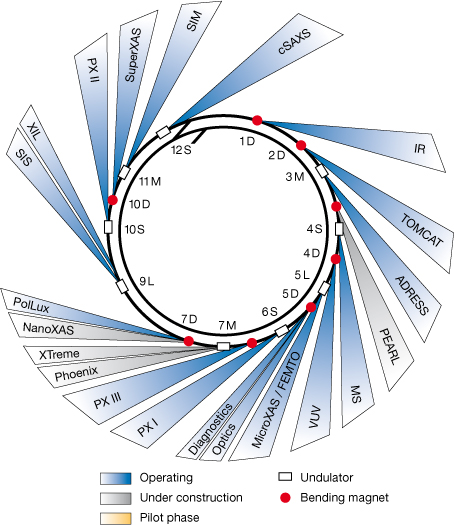
\includegraphics[width=\imsize]{img/SLS_beamlines_2008}
	\caption{Beamlines at the Swiss Light Source. Image from the \href{http://sls.web.psi.ch/view.php/beamlines/}{SLS Website}}
	\label{fig:beamlines}
\end{figure}

\section{TOMCAT}
A detailed explanation of the beamline for \acf{TOMCAT}, where all the tomography data for this thesis has been presented by \citet{Stampanoni2006a}.

As a short rundown the most important features of the beamline are presented here 

\renewcommand{\imsize}{0.5\linewidth}
\begin{figure}[htb]
	\subfloat[Overview of the Imaging Setup: The blue structure behind the control laptop is the sample stage. The black structure above contains the scintillator, the microscope optics and the camera.]{%
		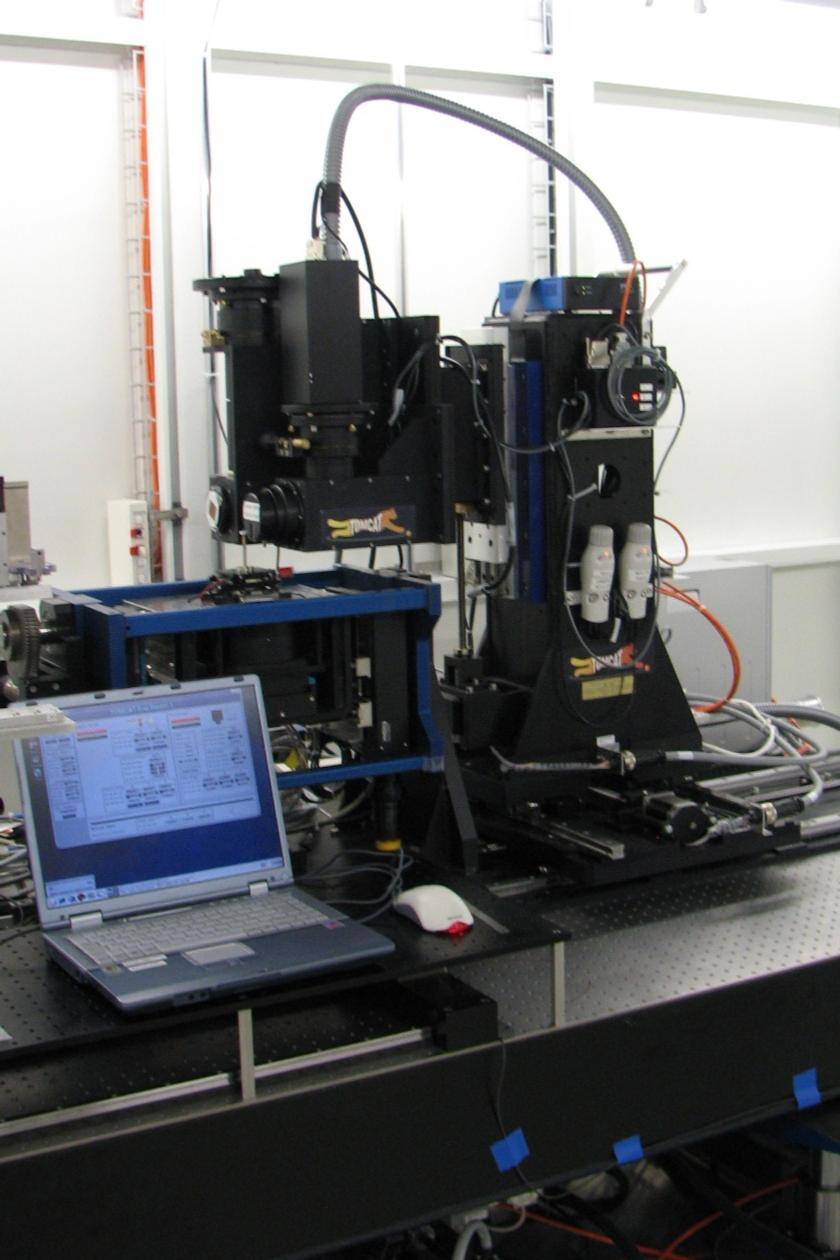
\includegraphics[width=\imsize]{img/TOMCAT1}%
		\label{subfig:TOMCAT1}%
		}%
	\subfloat[Close up view of a sample installed in front of the scintillator and microscope optics.]{%
		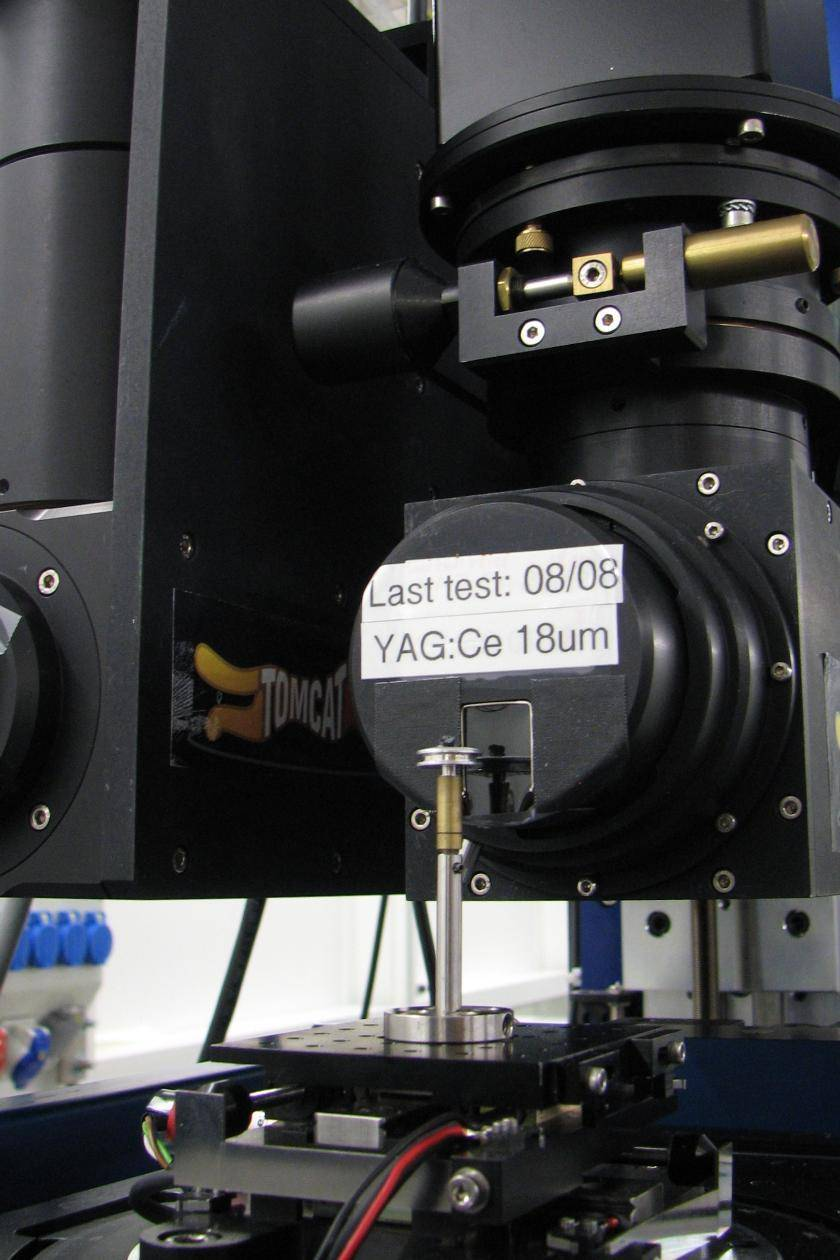
\includegraphics[width=\imsize]{img/TOMCAT2}%
		\label{subfig:TOMCAT2}%
		}%
	\caption{Images of the \ac{TOMCAT} beamline.}
\end{figure}

\begin{itemize}
	\item Beam
    \item Sample Handling
    \item Data Acquisition
    \item Reconstruction
\end{itemize}